
\subsection{Statement}

Let $L > 0$ be a constant and consider the square domain $\Omega = (0,L) \times
(0,L) \subset \real^2$. In $\Omega$ we consider the steady state version of the
generalized convection--diffusion equation
\eqref{eq:cde_general_convection_diffusion_equation}, with no source term,
constant density and constant diffusion coefficient, that is to say,
\begin{equation*}
	\frac{\rho}{\Gamma} \vb{v} \vdot \grad{\phi} = \Delta{\phi}
\end{equation*}
The following Dirichlet boundary conditions are prescribed:
\begin{itemize}[topsep=0pt]
	\item $\phi = \phi_\text{low}$ on $C_1 = [0,L) \times \{ 0 \} \cup \{ L \}
	\times [0,L)$.
	\item $\phi = \phi_\text{high}$ on $C_2 = \{ 0 \} \times (0,L] \cup (0,L]
	\times \{ L \}$.
\end{itemize}
Notice that $C_1, \ C_2 \subset \real^2$ constitute a partition of the boundary
of $\Omega$. In order to encode the boundary conditions more easily, we define
the function $g \colon \overline{\Omega} \rightarrow \real$ in the following way:
\begin{equation*}
	g(x,y) =
	\left\{
	\begin{aligned}
		&\phi_\text{low} 	& &\text{if } (x,y) \in C_1 \\
		&\phi_\text{high} 	& &\text{if } (x,y) \in C_2 \\
		&0					& &\text{if } (x,y) \in \Omega
	\end{aligned}
	\right.
\end{equation*}
The velocity field is $\vb{v} = v_0 \cos(\alpha) \vb{i} + v_0 \sin(\alpha)
\vb{j}$ with $v_0 > 0$ constant and $\alpha = \pi / 4$, whence
\begin{equation*}
	\frac{\rho}{\Gamma} \vb{v} \vdot \grad{\phi} = 
	\frac{\rho v_0 \cos(\alpha)}{\Gamma} \left( \phi_x + \phi_y \right) = 
	\underbrace{\frac{\cos(\alpha)}{L}}_{\beta} 
	\underbrace{\frac{\rho v_0 L}{\Gamma}}_{\peclet} \left( \phi_x + \phi_y \right) = 
	\left( \phi_x + \phi_y \right) \beta \, \peclet 
\end{equation*}
The resulting Cauchy problem is gathered in
\eqref{eq:diagonal_case_cauchy_problem} and summarized in figure
\ref{fig:diagonal_case_cauchy_problem}.
\begin{equation} \label{eq:diagonal_case_cauchy_problem}
	\left\{
	\begin{aligned}
		\Delta \phi - \left( \phi_x + \phi_y \right) \beta \, \peclet &= 0 &
		&\text{in } \Omega \\
		\phi &= g &
		&\text{on } \partial \Omega
	\end{aligned}
	\right.
\end{equation}
\begin{figure}[h]
	\centering
	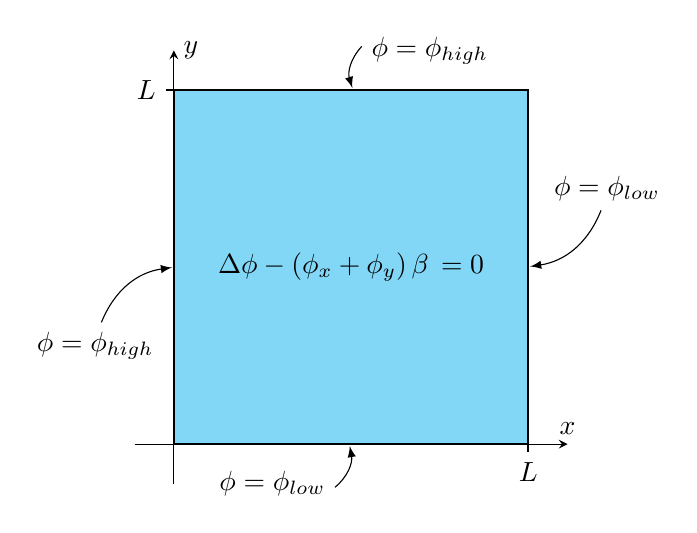
\begin{tikzpicture}
		% Lenghts
		\def\alength{5}
		\def\L{4.5}
		\def\mlength{0.1}
		% Axis
		\draw[-stealth] (0,-0.5) -- (0,\alength) node[right]{$y$};
		\draw[-stealth] (-0.5,0) -- (\alength,0) node[above]{$x$};
		\draw[black, thick] (\L,0) -- ++(0,-\mlength) node[below]{$L$};
		\draw[black, thick] (0,\L) -- ++(-\mlength,0) node[left]{$L$};
		% Domain
		\fill[cyan!70!white,opacity=0.7] (0,0) rectangle (\L, \L);
		\draw[thick, thick] (0,0) rectangle (\L, \L);
		% Right boundary condition
		\node[inner sep=0pt] at (\L,{0.5*\L}) (rb) {};
		\node[] at ({\L+1},{0.5*\L+1}) (rbc) {$\phi = \phi_\text{low}$};
		\path[-latex] (rbc) edge[bend left] node [left] {} (rb);
		% Top boundary condition
		\node[inner sep=0pt] at ({0.5*\L},\L) (tb) {};
		\node[] at ({0.5*\L+1},{\L+0.5}) (tbc) {$\phi = \phi_\text{high}$};
		\path[-latex] (tbc) edge[bend right] node [left] {} (tb);
		% Left boundary condition
		\node[inner sep=0pt] at (0,{0.5*\L}) (lb) {};
		\node[] at (-1,{0.5*\L-1}) (lbc) {$\phi = \phi_\text{high}$};
		\path[-latex] (lbc) edge[bend left] node [left] {} (lb);
		% Bottom boundary condition
		\node[inner sep=0pt] at ({0.5*\L},0) (bb) {};
		\node[] at ({0.5*\L-1},-0.5) (bbc) {$\phi = \phi_\text{low}$};
		\path[-latex] (bbc) edge[bend right] node [left] {} (bb);
		% PDE
		\node[] at ({0.5*\L},{0.5*\L}) 
		{$\Delta \phi - \left( \phi_x + \phi_y \right) \beta \, \peclet = 0$};
	\end{tikzpicture}
	\caption{Cauchy problem for the diagonal flow case.}
	\label{fig:diagonal_case_cauchy_problem}
\end{figure}

\noindent



